
\documentclass[conference]{IEEEtran}
\usepackage{cite}
\usepackage{amsmath,amssymb,amsfonts}
\usepackage{graphicx}
\usepackage{textcomp}
\usepackage{xcolor}
\usepackage{multicol}
\usepackage{float}
\usepackage[spanish]{babel}
\usepackage[spanish,vlined,ruled,]{algorithm2e}

\def\BibTeX{{\rm B\kern-.05em{\sc i\kern-.025em b}\kern-.08em
    T\kern-.1667em\lower.7ex\hbox{E}\kern-.125emX}}
\begin{document}

\title{Imagenes Panorámicas}
\author{\IEEEauthorblockN{Joaquín Pérez Araya}
\IEEEauthorblockA{\textit{Departamento de Ciencias de la Computación} \\
\textit{Universidad de Chile}\\
Santiago, Chile \\
joaquin.perez.a@ug.uchile.cl}}


\maketitle

\begin{abstract}
    Se usan histogramas de orientaciones para obtener recuperar imágenes a traves de dibujos de consultas.
\end{abstract}
 

\section*{Introducción} % ***Así la cosa no me molesta con los numeritos***
    Dentro del ámbito de análisis de imágenes, existen medidas que permiten caracterizar una imagen en particular, por ejemplo un histograma de colores de una imágen. Ëstas medidas se pueden clasificar en dos tipos, globales, que utilizan la información completa de la imagen (como el ejemplo anterior) y, por otra parte, los descriptores locales que describen áreas importantes dentro de ésta, así como elementos principales de ésta, etc.
    En este documento se utilizará el descriptor local SIFT para encontrar similitudes entre dos imágenes, para unirlas generando una imagen panorámica usando ambas imágenes.
    Para lograr este fín se utilizará el descritor local SIFT para encontrar 
    

    Para es estudio de imágenes uno de los descriptores de imagen útiles es el histograma de orientaciones, es decir, un histograma de los ángulos internos de ésta. En este documento se mencionará la implementación y funcionamiento de 3 formas de cálculo de histogramas de orientación, uno que calula los ángulos por pixel, otro que divide la imagen en bloques de un tamaño fijo para despues calcular los ángulos en cada bloque (HELO) y finalmente el último que divide la imagen en bloque y calcula los ángulos utilizando interpolación lineal según la posición de cada pixel del bloque (SHELO).
    
    Una de las posibles usos de este tipo de histogramas es en el ámbito de la recuperación de imágenes por dibujos, que dado un dibujo simple (como los que se puede hacer con una hoja y lápiz), obtener imagenes que representen el dibujo dado.
    
\begin{figure}[H]
\begin{multicols}{4}
    \centering
    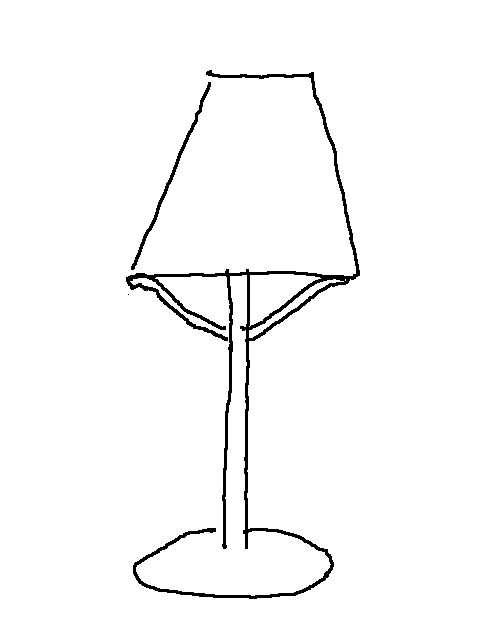
\includegraphics[width=0.95\linewidth]{image/lamps.jpg} \par
    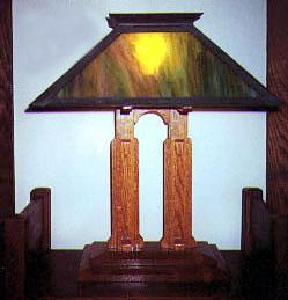
\includegraphics[width=0.95\linewidth]{image/lamp1.jpg} \par
    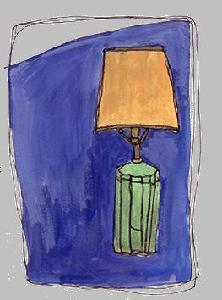
\includegraphics[width=0.95\linewidth]{image/lamp2.jpg} \par
    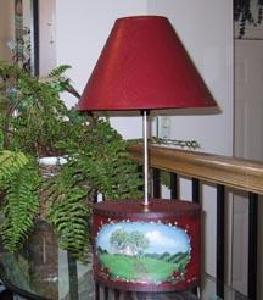
\includegraphics[width=0.95\linewidth]{image/lamp3.jpg} \par
\end{multicols}
\caption{Ejemplo de una posible búsqueda, la imagen de la izquierda representa el dibujo de búsqueda y las de la derecha los resultados esperados.}
\end{figure}
    
    Para resolver este problema, los histogramas de orientaciones son muy útiles, ya que dado dos imágenes con objetos del mismo tipo, es muy probable que tengan dentro formas similares, y un histograma de orientaciones contalibiza esa idea abstracta de similitud entre imágenes.
    
\section*{Diseño e Implementación}
	La implementación realizada se divide en dos partes, los histogramas y las consultas.
\subsection*{Histogramas}
	Para el diseño e implementación de los tres histogramas se creó la función auxiliar $ConvolveSobel$ que calcula el gradiente en ambas direcciones utilizando la máscara Sobel. La implementación utiliza el siguiente algoritmo: 

\begin{algorithm}[ht]
	\caption{ConvolveSobel}	
	\KwData{$image$ un arreglo que representa la imagen.}
	\KwResult{Gradientes en X e Y de $imagen$, usando Sobel.}
	\DontPrintSemicolon
	\Begin{
	$Sobel_x \longleftarrow 
	\{ \{-1,0,1\}, \{-2,0,2\}, \{-1,0,1\} \}			
			$\;
	$Sobel_y \longleftarrow transpose(Sobel\_x)$\;

	$G_x \longleftarrow convolve(image,Sobel_x) $\;
	$G_y \longleftarrow convolve(image,Sobel_y) $\;
	\KwRet{$G_x, \; G_y$}
	}
	Notar que $transpose()$ es la operación trasponer y $convolve()$ es la convolución de matrices.
\end{algorithm}


\subsubsection*{Histograma de Orientaciones Simple}
	En este histograma se calculan los ángulos por cada pixel de la imagen y luego se dividen dichos ángulos según las cubetas (bins) dado.
	\begin{algorithm}[ht]
		\caption{Histograma de Orientaciones Simple}	
		\KwData{$image$ un arreglo que representa la imagen, la cantidad de bins $k$.}
		\KwResult{Histograma de orientaciones de $image$.}
		\DontPrintSemicolon
		\Begin{
		$h \longleftarrow zeros(k)$ \;
		$G_x, G_y \longleftarrow ConvolveSobel(imagen)$\;

		$angles \longleftarrow arctan(\frac{G_x}{G_y})$\;
		\For{$angle$ in $angles$}{
			\If{$angle < 0$}{
				$angle \longleftarrow angle + \pi$\;			
			}		
		}
		$mag \longleftarrow \sqrt{G_x^2+G_y^2}$ \;
		$index \longleftarrow \lfloor \frac{angles}{\pi} (k-1)\rfloor mod \; k $ \;
		\For{$i= 0$ to $k$}{
			$r, c \longleftarrow indexes$ where $index(r,c) = i$ \;			$h[i] \longleftarrow \sum mag[r,c]$
		}
		$h \longleftarrow normalize(h,2)$ \;
		\KwRet{$h$}}
		
		\end{algorithm} 
	
	\begin{figure}[H]
    \centering
    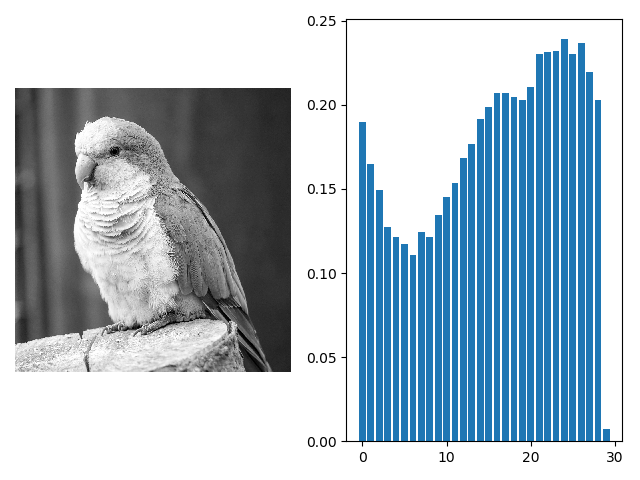
\includegraphics[width=0.95\linewidth]{image/birb_hist.png}
\caption{Imagen de una cotorra con su histograma de orientaciones simple, utilizando 30 bins.}
\end{figure}	

\subsubsection*{Histograma de Orientaciones de Bordes Locales (HELO)} 
Separa la imagen en bloques cuadrados de tamaño determinado, se calculan los ángulos por cada bloque, para luego separarlos en los diferentes cubetas.
    	\begin{algorithm}[ht]
		\caption{Histograma de Orientaciones de Bordes Locales}	
		\KwData{$image$ un arreglo que representa la imagen, la cantidad de bins $k$, tamaño de los bloques $B$.}
		\KwResult{Histograma de orientaciones de $image$.}
		\DontPrintSemicolon
		\Begin{
		$width \longleftarrow width(image)$ \;
		$height \longleftarrow height(image)$ \;
		$h \longleftarrow zeros(k)$ \;
		$(G_x, G_y) \longleftarrow ConvolveSobel(imagen)$\;
        $L_x, L_y \longleftarrow zeros((B+1,B+1))$\;
        \For{$(i,j)$ in $image$}{
            $r = round(\frac{ i * B}{height})$\;
            $s = round(\frac{ j * B}{width}$\;
            $L_x(r,s) += \sqrt{G_x(i,j) - G_y(i,j)} $\;
            $L_y(r,s) += 2(G_x(i,j)G_y(i,j))$ \;
        }
		$angles \longleftarrow arctan(\frac{L_y}{L_x})$\;
		\For{$angle$ in $angles$}{
			\If{$angle < 0$}{
				$angle \longleftarrow angle + \pi$\;			    $angle \longleftarrow angle * 0.5 $
			}		
		}
		$mag \longleftarrow \sqrt{G_x^2+G_y^2}$ \;
		$index \longleftarrow \lfloor \frac{angles}{\pi} (k-1)\rfloor mod \; k $ \;
		\For{$i= 0$ to $k$}{
			$r, c \longleftarrow indexes$ where $index = i$ \;			$h[i] \longleftarrow \sum mag[r,c]$
		}
		$h \longleftarrow normalize(h,2)$ \;
		\KwRet{$h$}}
		
		\end{algorithm} 	

	\begin{figure}[H]
    \centering
    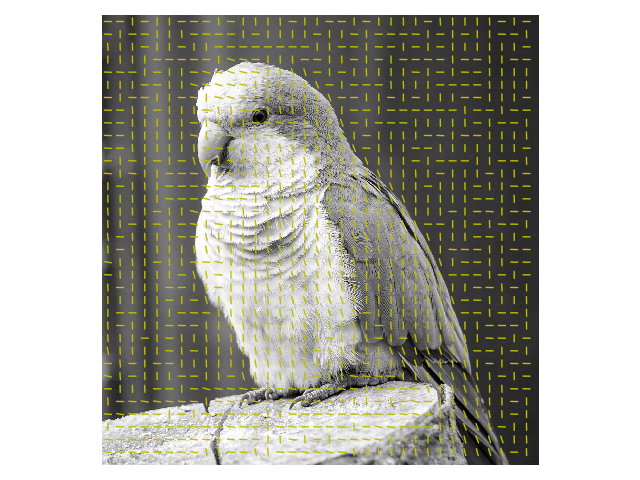
\includegraphics[width=0.95\linewidth]{image/birb_helo.png}
\caption{Imagen de una cotorra con su histograma de orientaciones locales (HELO), utilizando 35$\times$35 bloques.}
\end{figure}	
	
\subsubsection*{Histograma de Orientaciones de Bordes Locales Suave (SHELO)} 
     Posee la misma idea de implementación de HELO, sin embargo, SHELO adicionalmente interpola linealmente la ponderación de cada uno de los bloques según la cercanía que tiene el pixel que se está calculando. Así los pixeles de un bloque que están más en las fronteras de éste repartirán su peso en el histograma a los bloques cercanos.
    	\begin{algorithm}[ht]
		\caption{Histograma de Orientaciones de Bordes Locales Suave}	
		\KwData{$image$ un arreglo que representa la imagen, la cantidad de bins $k$, tamaño de los bloques $B$.}
		\KwResult{Histograma de orientaciones de $image$.}
		\DontPrintSemicolon
		\Begin{
		$width \longleftarrow width(image)$ \;
		$height \longleftarrow height(image)$ \;
		$h \longleftarrow zeros(k)$ \;
		$(G_x, G_y) \longleftarrow ConvolveSobel(imagen)$\;
        $L_x, L_y \longleftarrow zeros((B+1,B+1)$\;
        \For{$(i,j)$ in $image$}{
            $r = \frac{ i * B}{height} $\;
            $s = \frac{ j * B}{width} $\;
            $left \longleftarrow \lfloor s \rfloor$ \;  
            $right \longleftarrow min(left + 1, block - 1)$ \;  
            $bot \longleftarrow \lfloor r \rfloor$ \;  
            $top \longleftarrow min(bot + 1, block - 1)$ \;  
            $d_l \longleftarrow s - left - 0.5$ \;
            \If{$d_1$ < 0.5}{
               $w_l \longleftarrow d_l - 0.5$ \;
            }
            \Else{$w_l \longleftarrow 0.5 - d_l$ \;}
            $w_r \longleftarrow 1 - w_l$ \;
            
            $d_b \longleftarrow r - bot - 0.5$ \;
            \If{$d_b$ < 0.5}{
               $w_b \longleftarrow d_b - 0.5$ \;
            }
            \Else{$w_b \longleftarrow 0.5 - d_b$ \;}
            $w_t \longleftarrow 1 - w_b$ \;
            \For{hor, ver in $\{left, right\}\times \{top, bot\}$}{
                $L_x(hor,ver) += (\sqrt{G_x(i,j) - G_y(i,j)}) w(hor,ver)$\;
                $L_y(hor,ver) += 2(G_x(i,j)G_y(i,j)) w(hor,ver)$ \;
                }
            }
		$angles \longleftarrow arctan(\frac{L_x}{L_y})$\;
		\For{$angle$ in $angles$}{
			\If{$angle < 0$}{
				$angle \longleftarrow angle + \pi$\;			
			}		
		}
		$mag \longleftarrow \sqrt{G_x^2+G_y^2}$ \;
		$index \longleftarrow \lfloor \frac{angles}{\pi} (k-1)\rfloor mod \; k $ \;
		\For{$i= 0$ to $k$}{
			$r, c \longleftarrow indexes$ where $index = i$ \;			$h[i] \longleftarrow \sum mag[r,c]$
		}
		$h \longleftarrow normalize(h,2)$ \;
		\KwRet{$h$}}
		$w(hor,ver)$ es igual a ambos pesos $w_{hor}$ y $w_{ver}$ multiplicados.
		\end{algorithm} 	
	
	\begin{figure}[H]
    \centering
    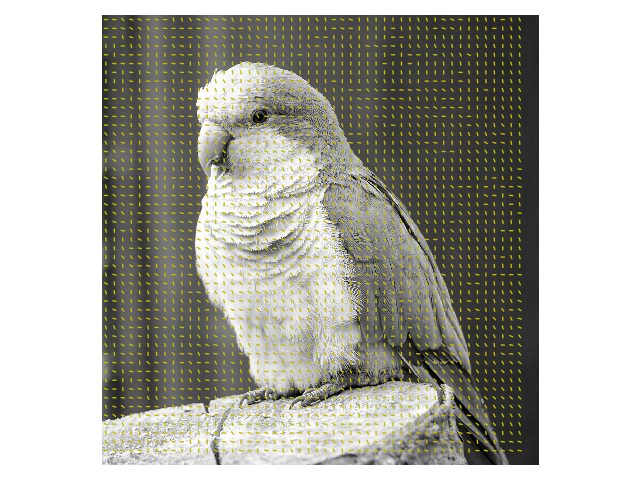
\includegraphics[width=0.95\linewidth]{image/birb_shelo50.png}
\caption{Imagen de una cotorra con su histograma de orientaciones local suave (SHELO), utilizando 50$\times$50 bloques.}
\end{figure}	
	
    Adicionalmente para cada método de cálculo de histograma, se creó una función que, dada una imagen, grafica las orientaciones por bloque en el caso de HELO y SHELO, o el histograma en el caso del normal.

	
\subsection*{Consultas}
    Para las consultas, se diseñaron distintas funciones para consultar a la base de dados dada, se utilizó la clase \texttt{ImageCollection} para almacenar y procesar las múltiples imágenes. \\
    Con la finalidad de reducir la carga del sistema al momento de hacer las consultas se implementó una función que aplica una función de histograma (\texttt{process\_database}) a todas las imágenes de la base de datos, ya que para diferentes imágenes de consulta, los histogramas son los mismos, sólo cambian si los parámetros de la función de cálculo del histograma cambia y la misma función cambia.
    También se diseño una función para buscar imágenes dentro de la base de datos, \texttt{sketch\_retrival}, que carga la base de datos y procede a retornar las matrices de las imágenes más relevantes hasta un número determinado por ésta. Esta función también tiene como argumentos la función de histograma, la cantidad de cubetas (bins) y la cantidad de bloques para evitar código duplicado.
    Finalmente se implementó la función \texttt{map\_query}, que calcula el mAP de una función de histograma con sus parámetros fijos leyendo una consulta y evaluando sus resultados con las tags (el nombre de la carpeta del archivo) para verificar la presición del método escogido.
    
\section*{Experimentación}
    Por temas de eficiencia de Python, utilizar todas las 1326 imágenes, haría que ejecutar la función de cálculo de mAP tomara bastante tiempo en calcular. Para las pruebas se utilizaron las consultas y las imágenes de la base de datos que empezaran con la letra A.
    Se utilizó la función \texttt{map\_query} para realizar la experimentación.

\begin{figure}[ht]
    \centering
    \begin{tabular}{|c|c|c|}
    \hline 
     & Sin Canny & Con Canny \\ 
    \hline 
    K=36 & 0.0330 & 0.0256 \\ 
    \hline 
    K=72 & 0.0295 & 0.0274 \\ 
    \hline 
    K=96 & 0.0275 & 0.0259 \\ 
    \hline 
    \end{tabular} 
\caption{mAP calculado utilizando el histograma simple.}    
    
\end{figure}
\section*{Conclusión}
    En términos de eficiencia, la función simple de histograma de orientaciones es excelente, sin embargo, su utilidad para la búsqueda de imágenes es pobre, cuyo rendimiento decrece según la cantidad de bins utilizado además de la bins utilizado, utilizar Canny en la imágenes de muestra hace menos precisa el método.


\begin{thebibliography}{99}
\bibitem{HELO} Saavedra J.M., Bustos B. (2010) An Improved Histogram of Edge Local Orientations for Sketch-Based Image Retrieval. In: Goesele M., Roth S., Kuijper A., Schiele B., Schindler K. (eds) Pattern Recognition. DAGM 2010. Lecture Notes in Computer Science, vol 6376. Springer, Berlin, Heidelberg.

\bibitem{SHELO}  Saavedra, J. (2014) SKETCH BASED IMAGE RETRIEVAL USING A SOFT COMPUTATION OF THE HISTOGRAM OF EDGE LOCAL ORIENTATIONS (S-HELO). ICIP

\end{thebibliography}

\section*{Anexo}

\end{document}
